% \subsection{SEM NOME} SUBSTITUIR AO FIM DO PROCESSO NAO ESQUECER!
% SUBSTITUIR ANGLICISMES téléchargé ...
% INSÉRER L'IMAGE
\part{De l'image au standard IIIF : conceptions des \eng{pipelines}}
\chapter{Optimisation des images et objets pour IIIF : outils et méthodes}
    Le standard IIIF a ouvert de nouvelles voies pour la gestion et la visualisation de contenus numériques, notamment les images 2D et les modèles 3D. Cependant, l'intégration harmonieuse de ces différents types de ressources au sein de ce cadre reste un défi. Si des applications spécifiques ont été développées pour répondre à cette problématique \footnote{Par exemple, l'emploi de GIMP, Blender et MeshLab pour cette tâche est déjà connu dans le milieu patrimoniale, Voir \cite{raemygautschy2023}.}, leurs limites en termes de flexibilité et de maintenance ont rapidement été mises en évidence. C'est dans ce contexte que des chercheurs se sont tournés vers des solutions plus automatisées, telles que les scripts Python \footnote{Dans son article de 2023, Rossenova constate également ce problème, et cite l'exemple du \eng{The Smithsonian Cook} comme tentative pour contourner ce défi. Voir \cite{rossenova2023iiif}. Bien que l'étude de Ioannides et Patias ne se concentre pas spécifiquement sur cette question, il est intéressant de noter que, bien que récente, elle évoque les difficultés liées à la manipulation de modèles 3D sans aborder la possibilité d'utiliser des scripts Python. Cet ouvrage constitue néanmoins une réflexion précieuse sur les défis rencontrés dans ce domaine. Voir \cite{ioannides_patias_2023}.}.

    Dans cette étude, nous nous proposons d'explorer plus en détail les possibilités offertes par les \eng{pipelines} automatisés en Python pour traiter les défis liés à l'intégration de contenus 2D et 3D au sein du standard IIIF. En s'appuyant sur les travaux existants, nous présenterons ces \eng{pipelines}, capables de s'adapter à une grande variété de données.
    
    \section{Conception du \cvt}
    \cvt est une application conçue pour convertir des images aux formats .jpg, .jpeg et .png en versions plus légères. Il visait remplacer le logiciel GIMP.
        \subsection{Bibliothèques}
        Ce code Python utilise plusieurs bibliothèques pour effectuer la conversion et le téléchargement d'images redimensionnées. Voici un aperçu de chacune d'entre elles :
        
        \subsubsection{Flask}
        
        \begin{lstlisting}[language=Python]
        from ..app import app, ALLOWED_EXTENSIONS
        \end{lstlisting}
        
        Importe l'application \FSK \texttt{app} et la variable \textbf{ALLOWED\_EXTENSIONS} depuis un module parent nommé \texttt{app}. Cette variable contient une liste d'extensions de fichiers d'images autorisés pour le traitement qui sont les suivants : \textbf{.jpg}, \textbf{.jpeg} et \textbf{.png}.
        
        \subsubsection{io}
        
        \begin{lstlisting}
        from io import BytesIO
        \end{lstlisting}
        
        Importe la classe BytesIO du module io. Cette classe permet de créer un objet ressemblant à un fichier en mémoire, ce qui est utile pour conserver temporairement l'image redimensionnée avant son téléchargement.
        
        \subsubsection{flask}
        \begin{lstlisting}
        from flask import render_template, redirect, request, url_for, send_file:
        \end{lstlisting}
        
        Importe plusieurs fonctions utiles de Flask pour la gestion des requêtes \textsc{HTTP}. Par exemple, \textbf{render}\textunderscore\textbf{template} permet de rendre des templates HTML pour l'affichage des pages \eng{web} ; \textbf{redirect} redirige l'utilisateur vers une autre URL ; \textbf{request}: Donne accès aux informations de la requête en cours, y compris les fichiers téléchargés ; \textbf{url}\textunderscore\textbf{for}: Génère l'URL d'un endpoint Flask en fonction de son nom ; finalement, \textbf{send}\textunderscore\textbf{file}: Permet de renvoyer un fichier à l'utilisateur en téléchargement.

        \subsubsection{werkzeug.utils}

        \begin{lstlisting}
        from werkzeug.utils import secure_filename
        \end{lstlisting}
        
        Importe la fonction \textbf{secure}\textunderscore\textbf{filename} du module werkzeug.utils. Cette fonction sécurise le nom de fichier téléchargé afin d'éviter des problèmes potentiels de sécurité.

        \subsubsection{Pillow}
        
        \begin{lstlisting}
        from PIL import Image
        \end{lstlisting}
        
        Importe la classe Image du module PIL (aussi connu sous le nom de Pillow). Cette bibliothèque est utilisée pour la manipulation d'images en \py.
        
        \subsection{Fonctionnalités du code}
        Le code \py implémente une application \eng{web} simple qui permet aux utilisateurs de télécharger une image et de la redimensionner avant de la télécharger à nouveau. Voici une explication détaillée des différentes parties du code :
        
        \subsubsection{Configuration globale (en dehors des fonctions)}

        \begin{lstlisting}
        Image.MAX_IMAGE_PIXELS = None
        \end{lstlisting}
        
        Supprime toute limite imposée par Pillow sur la taille maximale des images en \eng{pixels}.
        
        \subsubsection{Fonction \textbf{allowed\_file} (filename)}
        
        Vérifie si l'extension du fichier téléchargé correspond à l'une des extensions autorisées conservées dans la variable \textbf{ALLOWED\_EXTENSIONS}.
        
        \subsubsection{Fonction \textbf{resize}\textunderscore\textbf{image}()}
        
        Ouvre l'image en utilisant le nom de fichier \textbf{filename} fourni. Calcule le rapport de réduction nécessaire pour que l'image ne dépasse pas les dimensions maximales définies par \textbf{max}\textunderscore\textbf{width} et \textbf{max}\textunderscore\textbf{height} (ici 1024x1024 \eng{pixels}).
        
        Redimensionne l'image en utilisant le filtre anti-aliasing \textsc{Lanczos} pour une meilleure qualité.
        Renvoie l'image redimensionnée.

        \subsubsection{Route @app.route("/")}

        Correspond à la racine de l'application.
        Renvoie le template \html principal conservé dans le dossier pages/main.html. Ce template est responsable de l'affichage du formulaire de téléchargement de l'image.

        \subsubsection{Route @app.route("/convert", methods=['POST'])}

        Correspond à l'URL /convert et ne gère que les requêtes \textsc{HTTP} de type POST (souvent utilisées pour les formulaires de téléchargement).
        Exécute la fonction \textbf{upload}\textunderscore\textbf{image} pour traiter le fichier téléchargé.
        
        \subsubsection{Fonction \texttt{upload\_image}()}
        
        Vérifie si le formulaire de téléchargement contient un fichier nommé "file". Si aucun fichier n'est présent, redirige l'utilisateur vers la même page.
        Récupère le fichier téléchargé depuis la requête et vérifie si son nom n'est pas vide. 
        Si le fichier est valide et son extension est autorisée (vérification par \texttt{allowed\_file}), sécurise le nom de fichier et récupère son extension.
        Redimensionne l'image en utilisant la fonction \texttt{resize\_image}.
        Crée un objet BytesIO pour conserver l'image redimensionnée en mémoire.
        Enregistre l'image redimensionnée dans l'objet.
        
    \section{Conception du \msh}
    \msh est une application conçue pour convertir des images 3D en versions plus légères à l'aide d'une méthode de simplification par décimation quadratique des arêtes, similaire à celle disponible dans des logiciels comme MeshLab.
    
        \subsection{Bibliothèques}
        
        Dans le cadre de cette étude, l'objectif était de développer une méthode permettant de réduire la taille des modèles 3D. Pour ce faire, le prérequis était de trouver une bibliothèque qui utilise la méthode de contraction \eng{Method Iterative Contraction Edges with Quadric Error Metrics}, telle qu'implémentée dans l'outil MeshLab. Cette technique, détaillée dans l'article de Garland et Heckbert, consiste à simplifier progressivement un maillage en contractant les arêtes les moins significatives \footnote{Cet algorithme est le développement d'un algorithme précédent, créé aussi pour les auteurs en 1997, dans lequel ils se sont intéressés seulement par la réduction de surfaces. Il est donc intéressant de souligner que cet article les auteurs ont envisagé bien les problèmes des modèles 3D : 
        ils souvent présentent d'autres propriétés, telles les couleurs, textures et surface normales, qui ont été finalement traitées en 1998. De plus, en effet l'usage de mémoire est réduite comme ils ont prévu. Pour l'article de 1997, Voir \cite{garland1997surface}. Pour l'article de 1998 sur le \eng{Method Iterative Contraction Edges with Quadric Error Metrics} qui sert de base à cette fonction utilisée sur MeshLab, PyMeshLab et Open3D, Voir \cite{garland1998quadric}.}.

        Afin de mettre en œuvre cette méthode, deux bibliothèques Python ont été étudiées : PyMeshLab et Open3D. Ces deux bibliothèques offrent des fonctionnalités de traitement de maillages 3D et font référence au méthode de contraction des arêtes pour les surfaces avec des couleurs et textures de 1998.

        Après une phase de tests comparatifs qui a eu lieu pendant trois semaines, la bibliothèque Open3D a été sélectionnée. En effet, PyMeshLab, bien que proposant un large éventail de fonctionnalités, s'est révélée peu performante sur des modèles de grande taille, entraînant des temps de calcul excessivement longs, et voire des boucles infinies.

        Open3D s'est avéré être une solution efficace pour réduire la complexité des modèles 3D. Les performances de cette bibliothèque seront analysées en détail dans la troisième partie de ce travail. Cependant, il convient de noter que Open3D ne permet pas de reproduire intégralement les paramètres de l'application MeshLab. Cette limitation restreint quelque peu la flexibilité de l'outil, bien que le cœur de l'algorithme de contraction des arêtes étant identique dans les deux bibliothèques, des résultats satisfaisants ont pu être obtenus. Finalement, voici une explication détaillée de chaque bibliothèque du code \textbf{main.py}:

        \subsubsection{Flask}

        \begin{lstlisting}
        from ..app import app, ALLOWED_EXTENSIONS
        \end{lstlisting}
        
        Importez l'application \FSK \texttt{app} et la variable \texttt{ALLOWED\_EXTENSIONS} depuis un module parent nommé \texttt{app}. Cette variable contient une liste d'extensions de fichiers d'images, de modèles 3D, de textures et de couleurs autorisés pour le traitement, qui sont les suivants : \textbf{.glb}, \textbf{.gltf}, \textbf{.jpg}, \textbf{.mtl}, \textbf{.obj}, \textbf{.ply}, \textbf{.png}, \textbf{.stl}, \textbf{.tiff}.

        \subsubsection{os}
        Non explicitement importée, mais utilisée dans la fonction \texttt{tempfile.\linebreak NamedTemporaryFile}. Fournit des fonctions pour interagir avec le système d'exploitation, telles que la création de fichiers temporaires.


        \subsubsection{io}
        
        \begin{lstlisting}
        import io
        \end{lstlisting}
        
        Importe le module io qui fournit des classes pour la manipulation de flux de données.

        \subsubsection{open3d}
        
        \begin{lstlisting}
        import open3d as o3d
        \end{lstlisting}
        
        Importe la bibliothèque open3d sous le alias o3d. Cette bibliothèque est essentielle pour le traitement de nuages de points et de maillages 3D. Elle permet de charger, manipuler, visualiser et exporter des données 3D. Dans cette étude, elle a été utilisée en combinaison avec la méthode de réduction de maillages \eng{Method Iterative Contraction Edges with Quadric Error Metrics}.

        \subsubsection{numpy}
        
        \begin{lstlisting}
        import numpy as np
        \end{lstlisting}
        
        Importe la bibliothèque \textsc{numpy} sous le alias np. \textbf{NumPy} est une bibliothèque fondamentale pour le calcul scientifique en \py. Elle fournit des structures de données multidimensionnelles (tableaux) et des fonctions efficaces pour les opérations matricielles et algébriques linéaires.

        \subsubsection{tempfile}
        
        \begin{lstlisting}
        import tempfile
        \end{lstlisting}
        
        Importe le module \texttt{tempfile} qui fournit des fonctions pour créer des fichiers temporaires.

        \subsubsection{flask}

        Importé à partir de \texttt{..app}, comme vu précédemment. Fournit des fonctionnalités pour la création d'applications \eng{web} en \py.

        \subsubsection{werkzeug.utils}

         Importé à partir de \texttt{..app}, comme vu précédemment. Fournit des utilitaires divers, dont la fonction \texttt{secure\_filename} utilisée pour sécuriser les noms de fichiers téléchargés.

        \subsection{Fonctionnalités du code}

        Ce code \py implémente une application \eng{web} qui permet aux utilisateurs de monter une image sur le site, la convertir en un maillage 3D simplifié et la renvoie en téléchargement.Voici une explication détaillée des différentes parties du code :

        \subsubsection{Fonction \texttt{allowed\_file}(filename)}
        Comme pour la fonction précédente, vérifie si l'extension du fichier mis en ligne correspond à l'une des extensions autorisées conservées dans la variable \texttt{ALLOWED\_EXTENSIONS}.

        \subsubsection{Fonction \texttt{simplify\_image}(filename)}

        \textbf{Création de fichier temporaire :}
        
        Utilise \texttt{tempfile.NamedTemporaryFile} pour créer un fichier temporaire avec l'extension \textbf{.obj}.
        Écrit le contenu du fichier téléchargé (représenté par \eng{filename}) dans le fichier temporaire. 
        Stocke le nom du fichier temporaire dans la variable \texttt{temp\_filename}.\\
        
        \textbf{Lecture du maillage :}
        
        Utilise la fonction \texttt{o3d.io.read\_triangle\_mesh} pour lire le fichier temporaire (considéré comme un maillage 3D au format \textbf{.obj}).
        Stocke le maillage lu dans la variable \texttt{mesh}.\\
        
        \textbf{Centrage du maillage :}
        
        Calcule la boîte englobante (bounding box) du maillage à l'aide de \texttt{mesh.get\linebreak\_axis\_aligned\_bounding\_box}.
        Récupère les coordonnées minimum et maximum de la boite englobante.
        Calcule le centre de la boite englobante.
        Calcule le vecteur de translation nécessaire pour déplacer le maillage vers son centre.
        Déplace le maillage en utilisant la fonction \textbf{mesh.translate}.\\
        
        \textbf{Simplification des maillages :}
        
        Utilise la fonction \textbf{mesh.simplify\_quadric\_decimation(number\linebreak\_of\_triangles}) pour simplifier le maillage. Le paramètre \texttt{target\_number\linebreak\_of\_triangles} est fixé à 65000 dans ce code. Cette fonction réduit le nombre de triangles du maillage en s'appuyant sur une méthode de décimation quadratique.\\
        
        \textbf{Calcul et rendu des normales :}
        
        Calcule les normales des sommets et des triangles du maillage simplifié à l'aide des fonctions \textbf{mesh\_simplified.compute\_vertex\_normals} et \textbf{mesh\_simplified.compute\_\linebreak triangle\_normals}. Les normales permettent d'obtenir un éclairage réaliste lors du rendu du maillage.\\
        
        \textbf{Sauvegarde du maillage simplifié :}
         
        Similaire à la création du fichier temporaire, il utilise \texttt{tempfile.\linebreak NamedTemporaryFile} pour créer un nouveau fichier temporaire avec l'extension \textbf{.obj}.
        Enregistre le maillage simplifié dans le fichier temporaire à l'aide de la fonction o3d.io.write

    
    \section{Structure de \cvt et \msh}
    Concernant la structure du code, les deux applications utilisent la même structure de dossiers avec de légères modifications adaptées à leur cas d'utilisation. Le modèle de dossiers de ces deux applications a été inspiré par celui proposé sur GitHub par Maxime Challon, l'un de mes professeurs à l'\enc \footnote{Voir \cite{challon_coursm2tnah_flask}.}. En ce qui concerne le code de \cvt, notre travail s'est bénéficié des idées de l'application PNG-to-JPEG \footnote{Voir \cite{herrera_2023_png_to_jpeg}.}.

    De plus, les deux applications sont publiées de manière privée sur mon propre GitHub et seront finalement rendues publiques une fois la soutenance de mémoire effectuée. Une autre étape consistera à mettre à disposition la version finale de ces applications sur le \eng{Docker Hub} de \dsc, qui, comme mentionné précédemment dans le Chapitre 4, sert à archiver et à mettre à disposition les applications développées par l'organisation.

    Concernant le \cvt, il est possible d'observer sa structure générale à partir de cette arborescence sur GitHub :

        % structure GitHub du \cvt
        \begin{figure}[h!]
            \centering
            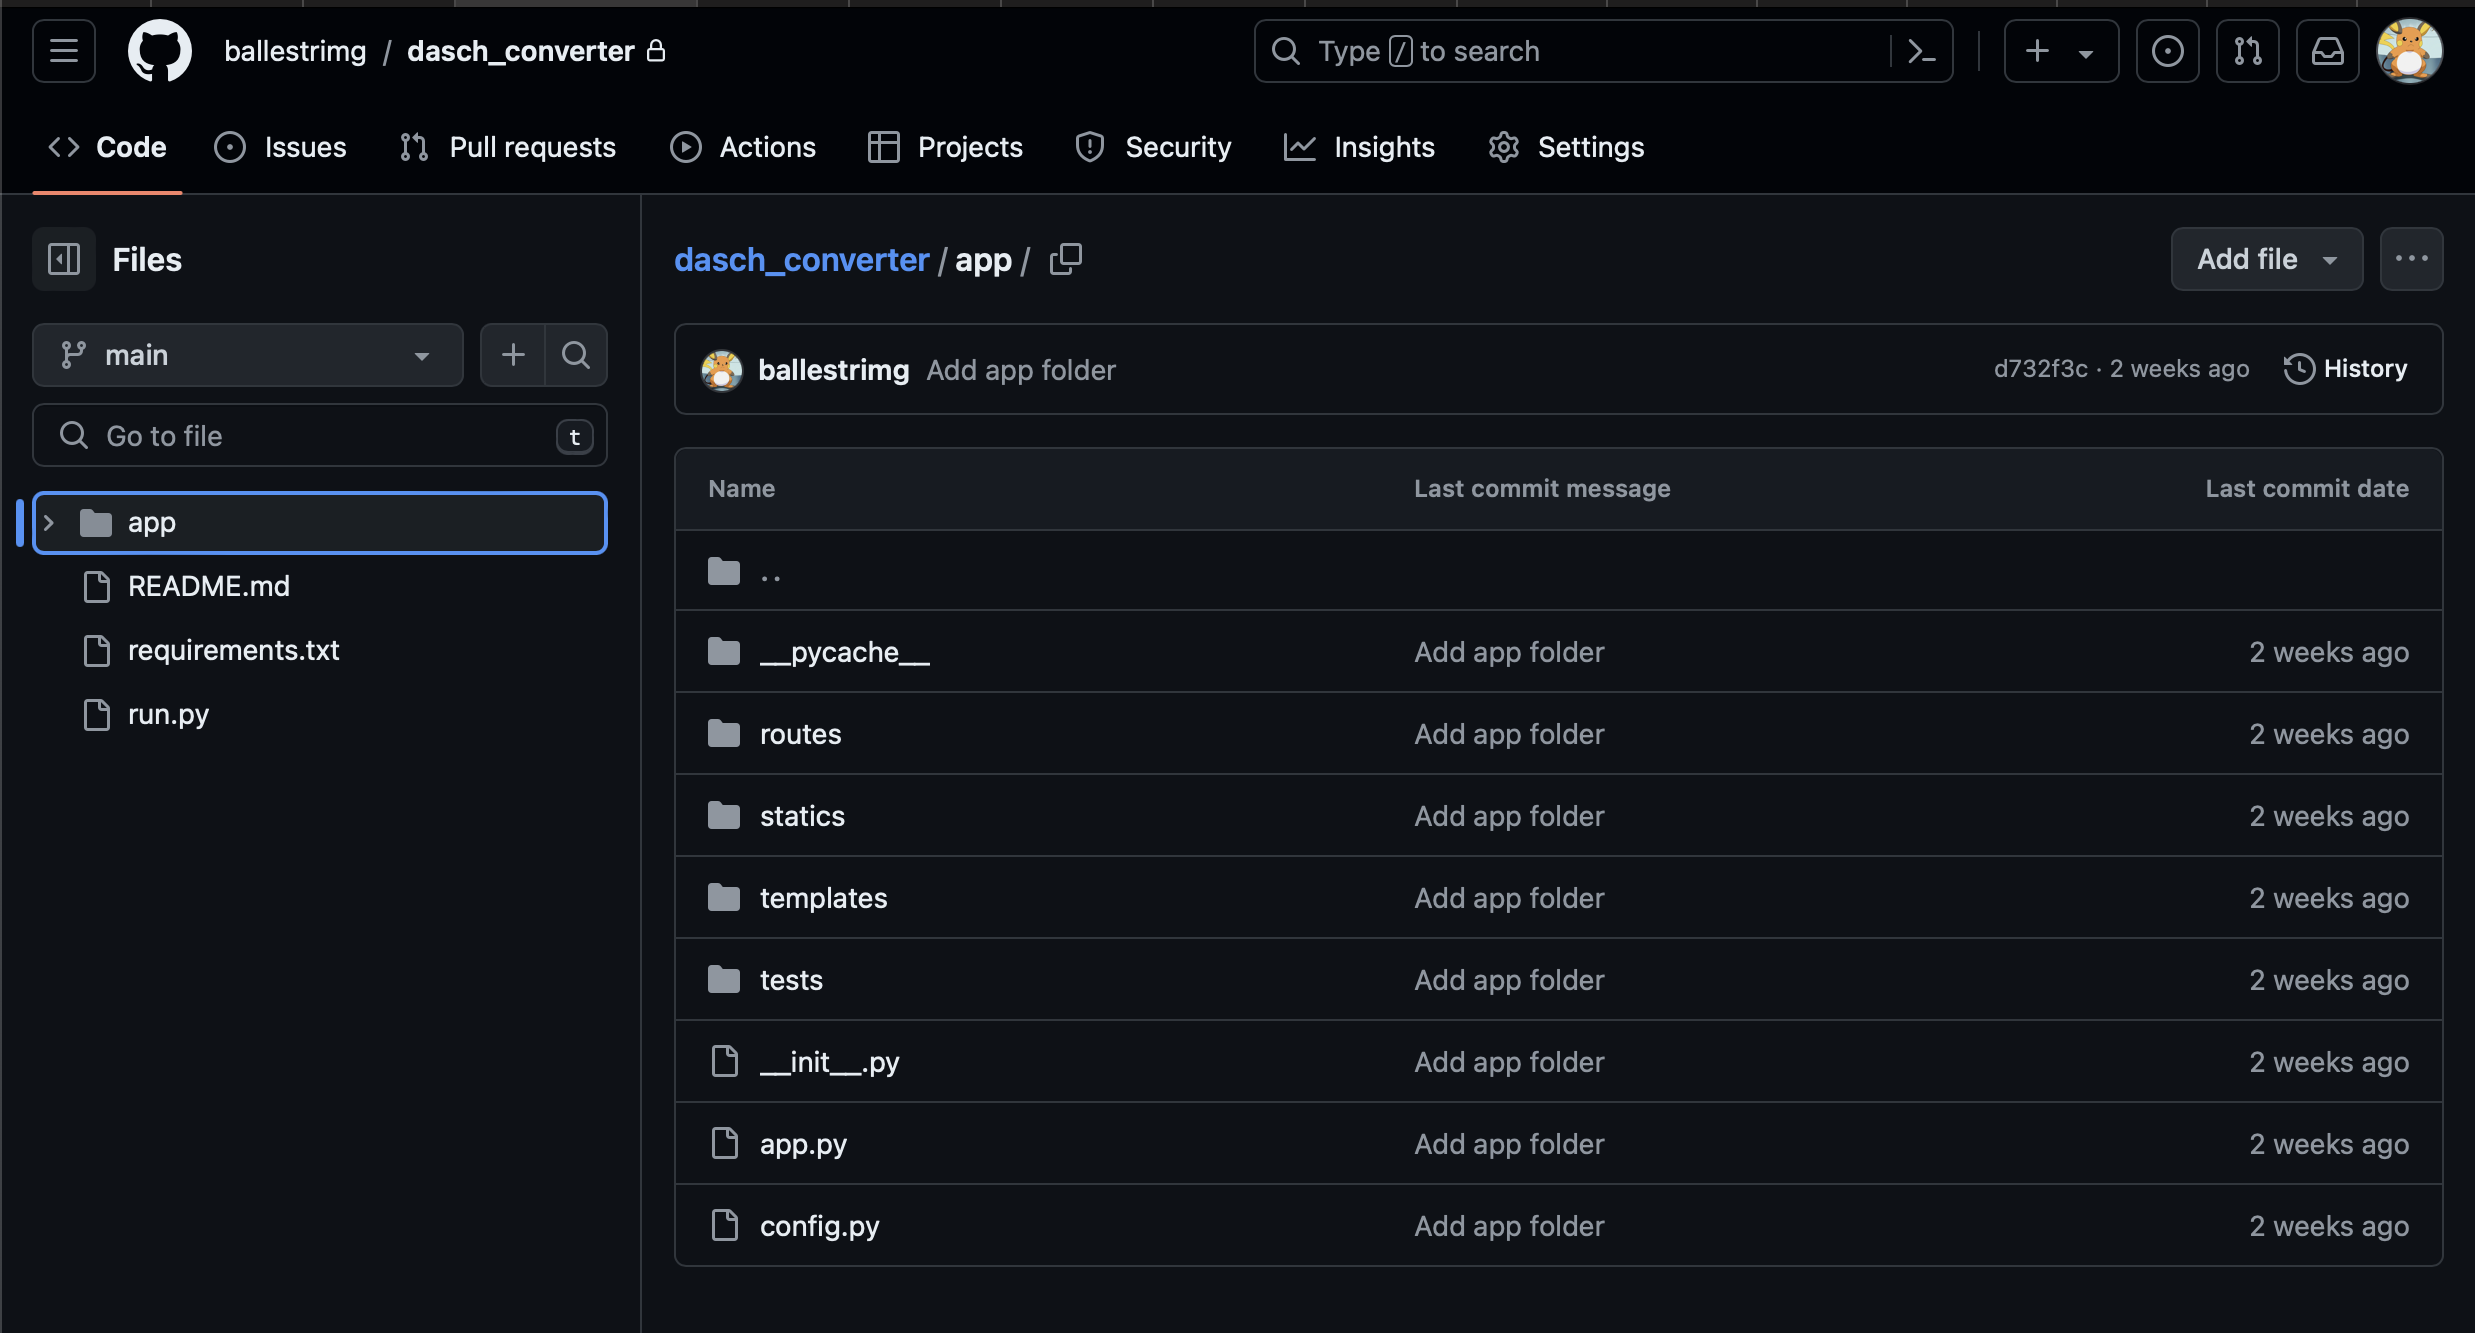
\includegraphics[width=12cm]{02_images/part_02/03_app_dasch_conv_github.png}
            \caption{Structure de l'application \cvt sur GitHub}
        \end{figure}

    Quant au \msh, sa structure est la suivante : 

    % structure GitHub du \msh
        \begin{figure}[h!]
            \centering
            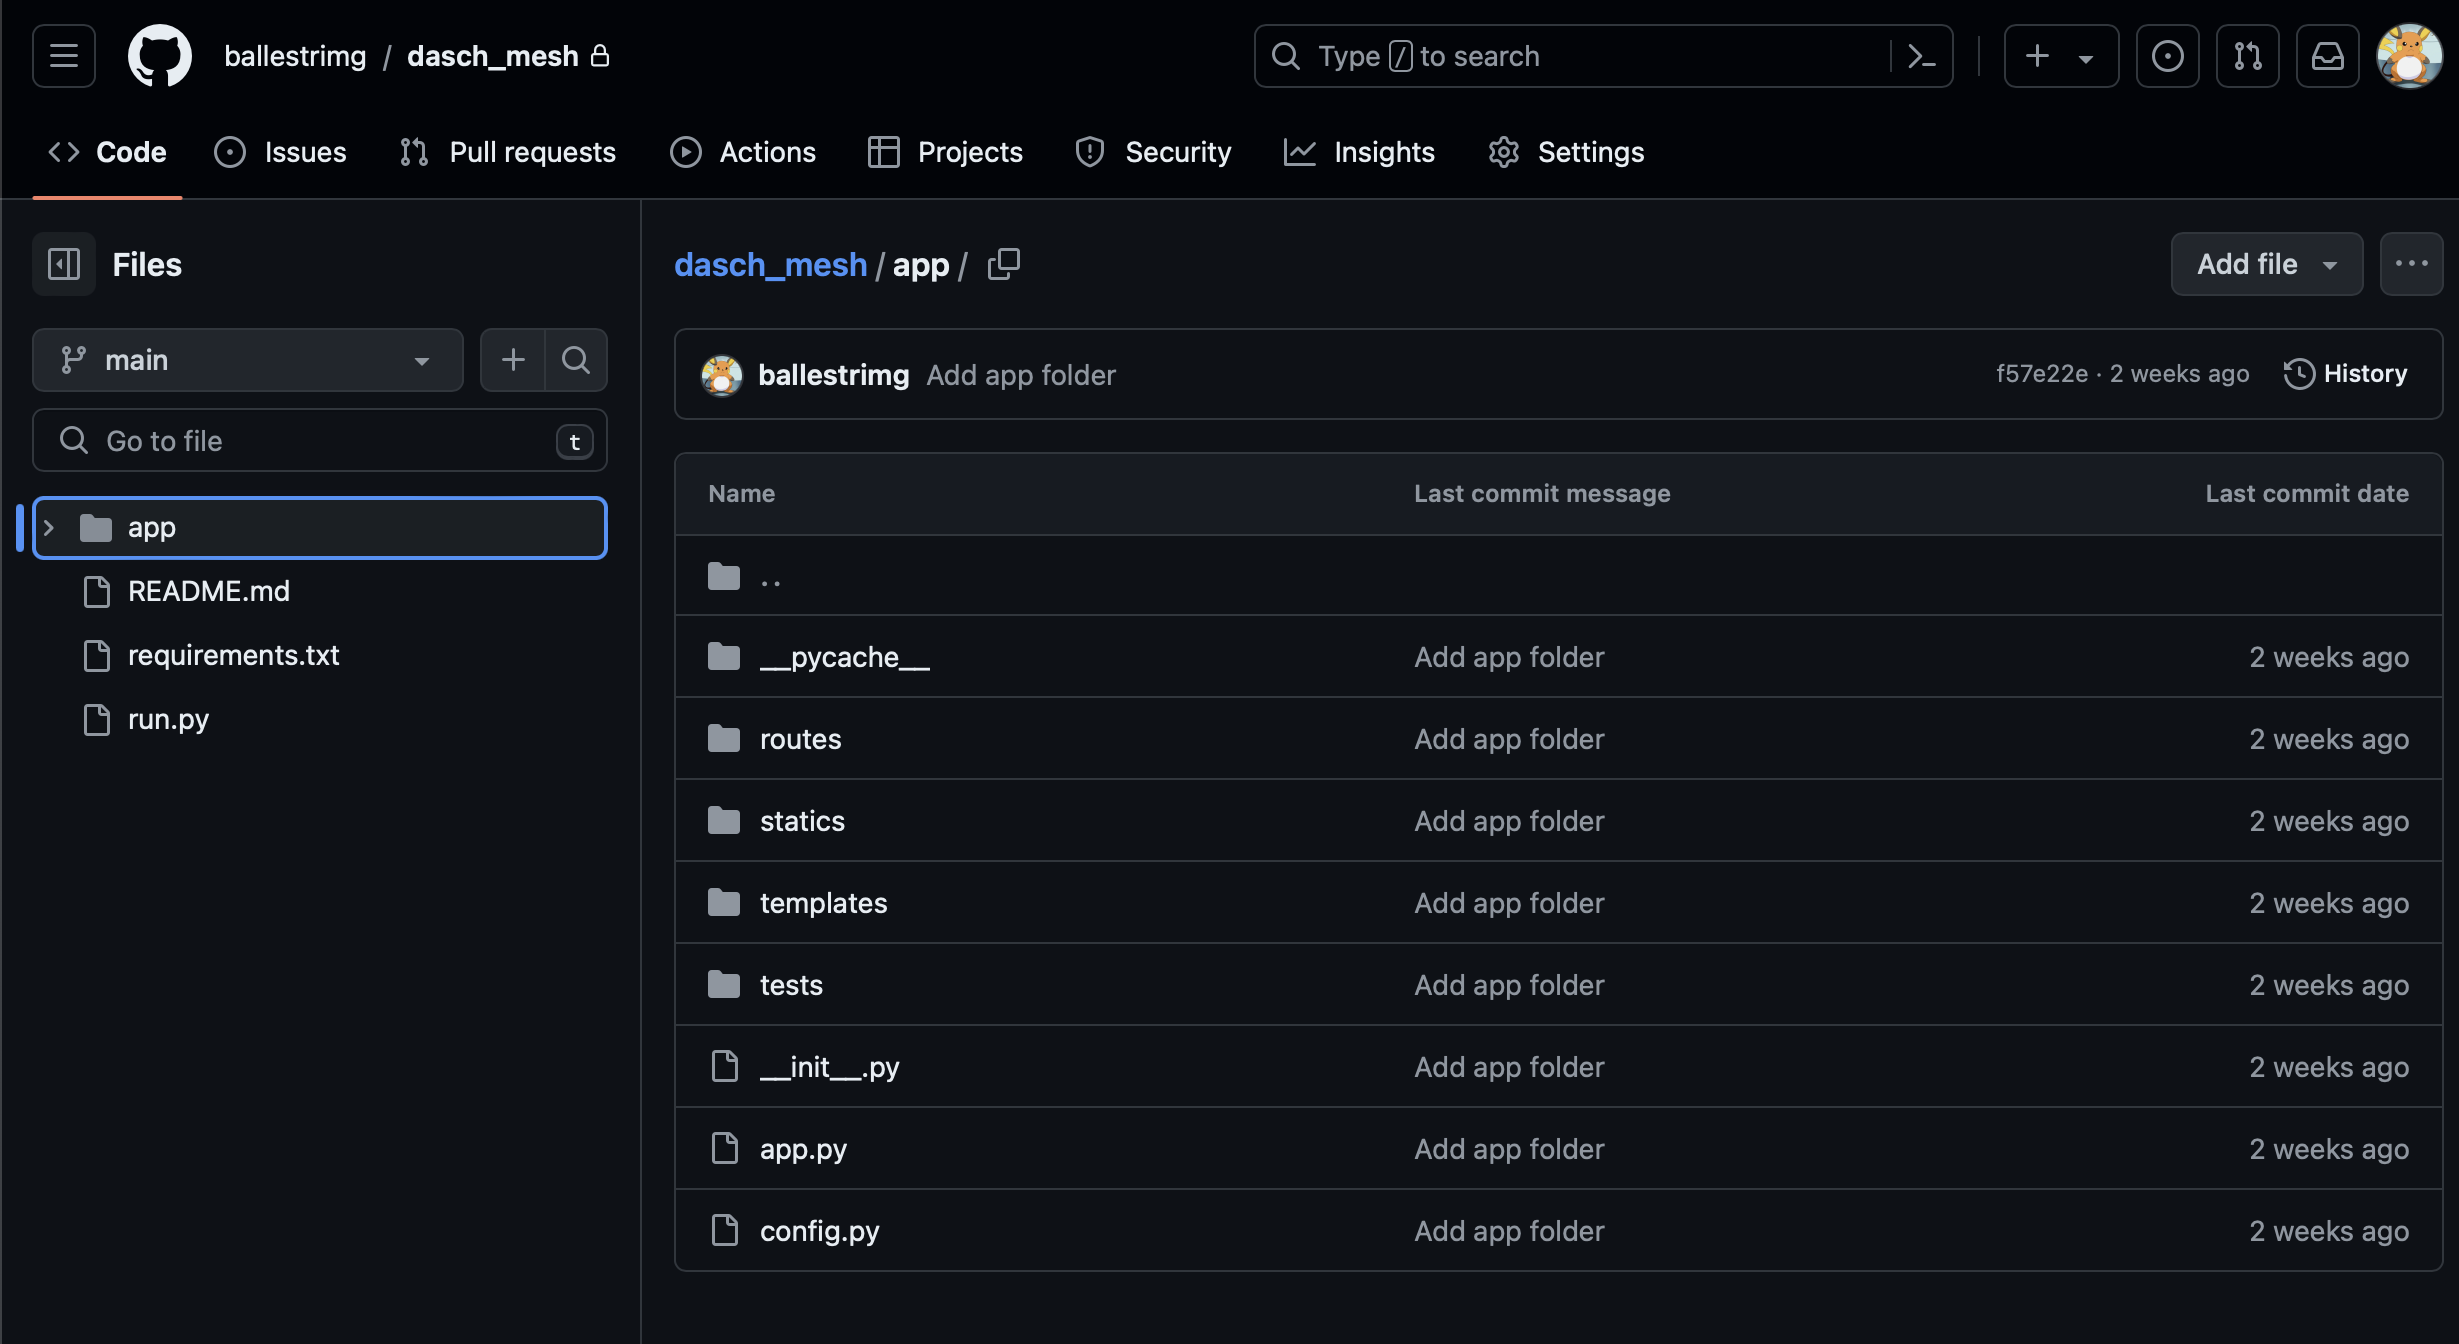
\includegraphics[width=12cm]{02_images/part_02/04_app_dasch_mesh_github.png}
            \caption{Structure de l'application \msh sur GitHub}
        \end{figure}

    L'arborescence des applications a pour but d'organiser les différents fichiers en dossiers, chacun correspondant à une fonctionnalité spécifique. Le dossier principal contient des sous-dossiers pour le code source, les tests, les données, la documentation et les fichiers de configuration. Cette structure permet une bonne séparation des préoccupations et facilite la maintenance du projet.
     
    Comme d'habitude pour les applications sur GitHub, on trouve un fichier \textbf{README.md} qui fournit une description du projet et un fichier \textbf{requirements.txt} qui liste les dépendances nécessaires pour exécuter l'application (bibliothèques, version Python, etc.). 

    Quant au \textit{design} de la page, il est inspiré du site \textbf{Smallpdf}. L'idée des boîtes pour y glisser des fichiers, ainsi qu'un bouton pour ajouter des contenus ont été utilisés en tant que principes des applications. 

        % structure GitHub du \msh
        \begin{figure}[h!]
            \centering
            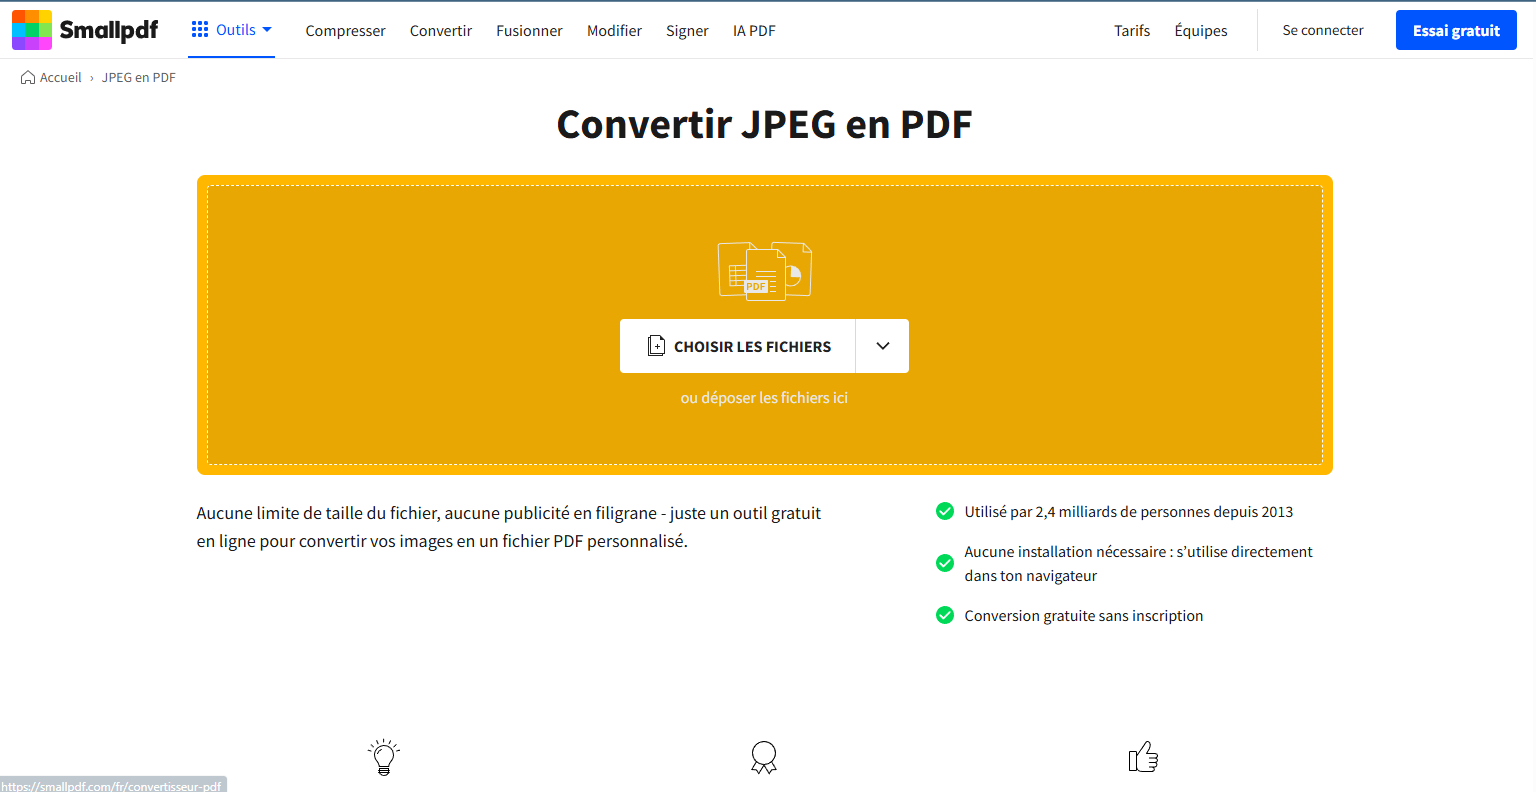
\includegraphics[width=12cm]{02_images/part_02/05_small_pdf.png}
            \caption{Page de convertion de fichier sur Smallpdf}
        \end{figure}
    
    Concernant les tests exécutés dans différentes versions \py, sur \eng{macOS M1} (\eng{Apple Silicon}) les versions \py pour \cvt et \msh ont été, respectivement, \textbf{3.11.0} et \textbf{3.9.0}~; sur \eng{Windows}, les deux applications ont utilisé la version \textbf{3.9.0} de \py~; les tests sur \eng{Ubuntu} \textbf{22.04.3} ont utilisé \py \textbf{3.10.12}. Il est important d'expliciter cela, car certaines bibliothèques comme \textsc{blinker 1.7.0} et \textsc{countourpy 1.2.1} n'acceptent pas des versions \py inférieures, respectivement, à \textbf{3.7.x} et \textbf{3.9.x}. De plus, jusqu'à ce jour, \textsc{open3d} fonctionne seulement dans les versions \py inférieures à \textbf{3.11.x}. A partir de Python 3.8, il est possible d'intégrer le framework Flask.

\chapter{Expérience utilisateur}
    \section{Intégration de l'UX dans les applications}
    
    Le développement de ces applications, \cvt et \msh, a mis en lumière l'importance de l'expérience utilisateur (\ux ou \eng{user experience}). Ce qui était autrefois perçu comme un domaine réservé aux designers s'est imposé comme un élément incontournable de la programmation, complétant la logique et le code de l'application. Dans ce chapitre, les raisons pour lesquelles l'intégration de l'\ux a été au cœur de nos préoccupations et comment il a été mis en œuvre seront discutés en détail.

    Pour mieux comprendre cette démarche, l'analyse abordera des différents aspects de l'application.

        \subsection{Vers une \ux inclusive}
        La conception d'applications numériques est souvent marquée par une dichotomie entre les utilisateurs experts, tels que les programmeurs et les administrateurs de plateformes, et les utilisateurs grand public, regroupant chercheurs, étudiants, amateurs et professionnels. Cette distinction, bien que pratique pour certains aspects de la conception, peut entraver la création d'une expérience utilisateur (\ux) véritablement inclusive. Or, en privilégiant un langage visuel efficace et en proposant une interface intuitive, notre application a cherché à combler ce fossé. En effet, en misant sur des éléments graphiques clairs et des interactions simples,  cet outil devient accessible à un large public, sans pour autant sacrifier les fonctionnalités attendues par les utilisateurs les plus expérimentés. Cette approche a permis de créer une expérience utilisateur unifiée, où les spécialistes peuvent tirer parti d'options avancées tout en offrant aux néophytes une prise en main rapide et efficace. Ainsi, en déconstruisant la traditionnelle opposition entre experts et grand public, notre application s'inscrit dans une démarche de démocratisation de l'accès aux outils numériques.

        \subsection{Fonctionnalités faciles à apprendre}
        Les deux applications ont été conçues pour répondre à un besoin spécifique : réduction de la taille des fichiers 2D et 3D. Pour atteindre cet objectif, les fonctionnalités simples et efficaces ont été mises en place, telles que le \eng{drag and drop} et les clics pour ajouter du contenu. Ces choix ont été guidés par le désir de minimiser la courbe d'apprentissage et de rendre l'application accessible à tous, y compris aux utilisateurs novices.

        \subsection{La palette de couleurs}
        La palette de couleurs a également été soigneusement sélectionnée. L'identité visuelle du \dsc a été maintenue tout en privilégiant des teintes qui ont la même couleur de l'association \footnote{De même pour la police de caractères \textsc{lato} \textsc{sans serif}, puisqu'elle est la police de \dsc.}. Les applications \cvt et \msh avaient, respectivement, les \eng{hex} couleurs \#336790 et \#74A2CF \footnote{Ces codes \eng{hex}, ainsi que les logos comme mentionné dans le Chapitre 2, ont été trouvés sur le document d'identité visuelle présent sur le compte Figma de \dsc. Il faut préciser que les codes de couleurs hexadécimaux, plus communément appelés codes \eng{Hex}, sont normalement composés d'un symbole dièse (\#) suivi de trois paires de chiffres représentant chacune les couleurs primaires RVB (rouge, vert, bleu). \cite{adobe_hex_codes}.}. Le choix de la couleur bleue avec peu de luminosité a deux raisons principales : en premier lieu, cette couleur est souvent associée dans notre culture à des entreprises reconnues telles qu'\eng{IBM} et \eng{Facebook} ; en deuxième lieu, sa basse luminosité et saturation suscitent plus d'émotions \footnote {Une étude menée avec des personnes de différentes cultures et niveaux de scolarité, fait pendant plusieurs années, a montré que la signification d'une couleur est plutôt influencé par sa luminosité et sa saturation et peu par sa teinte. C'est-à-dire qu'il n'y a pas une émotion liée de forme indissociable à une couleur à cause de sa teinte. Cela réfute l'idée reçue dans le design et la mode selon laquelle il y aurait une émotion universelle qui pourrait être associée à une couleur. En outre, pour les couleurs chaudes (\eng{warm-cool}) bien que la saturation et la teinte aient leur degré d'importance, les personnes n'avaient pas une opinion consistante sur quel aspect était le plus important, Voir \cite{crosscultemo}. Il est aussi intéressant de mentionner qu'une autre étude, plus ancienne, a déjà remarqué le fait que la perception visuelle est tellement complexe que d'autres aspects de nature distincte de la vision pourraient aussi jouer, tels que le goût, l'odeur et l'ambiance. Cela montre, encore une fois, l'importance de l'interdisciplinarité dans les champs d'études, Voir \cite{valberg2005}.}.

        % home page \cvt et \msh
        \begin{figure}[h!]
            \centering
            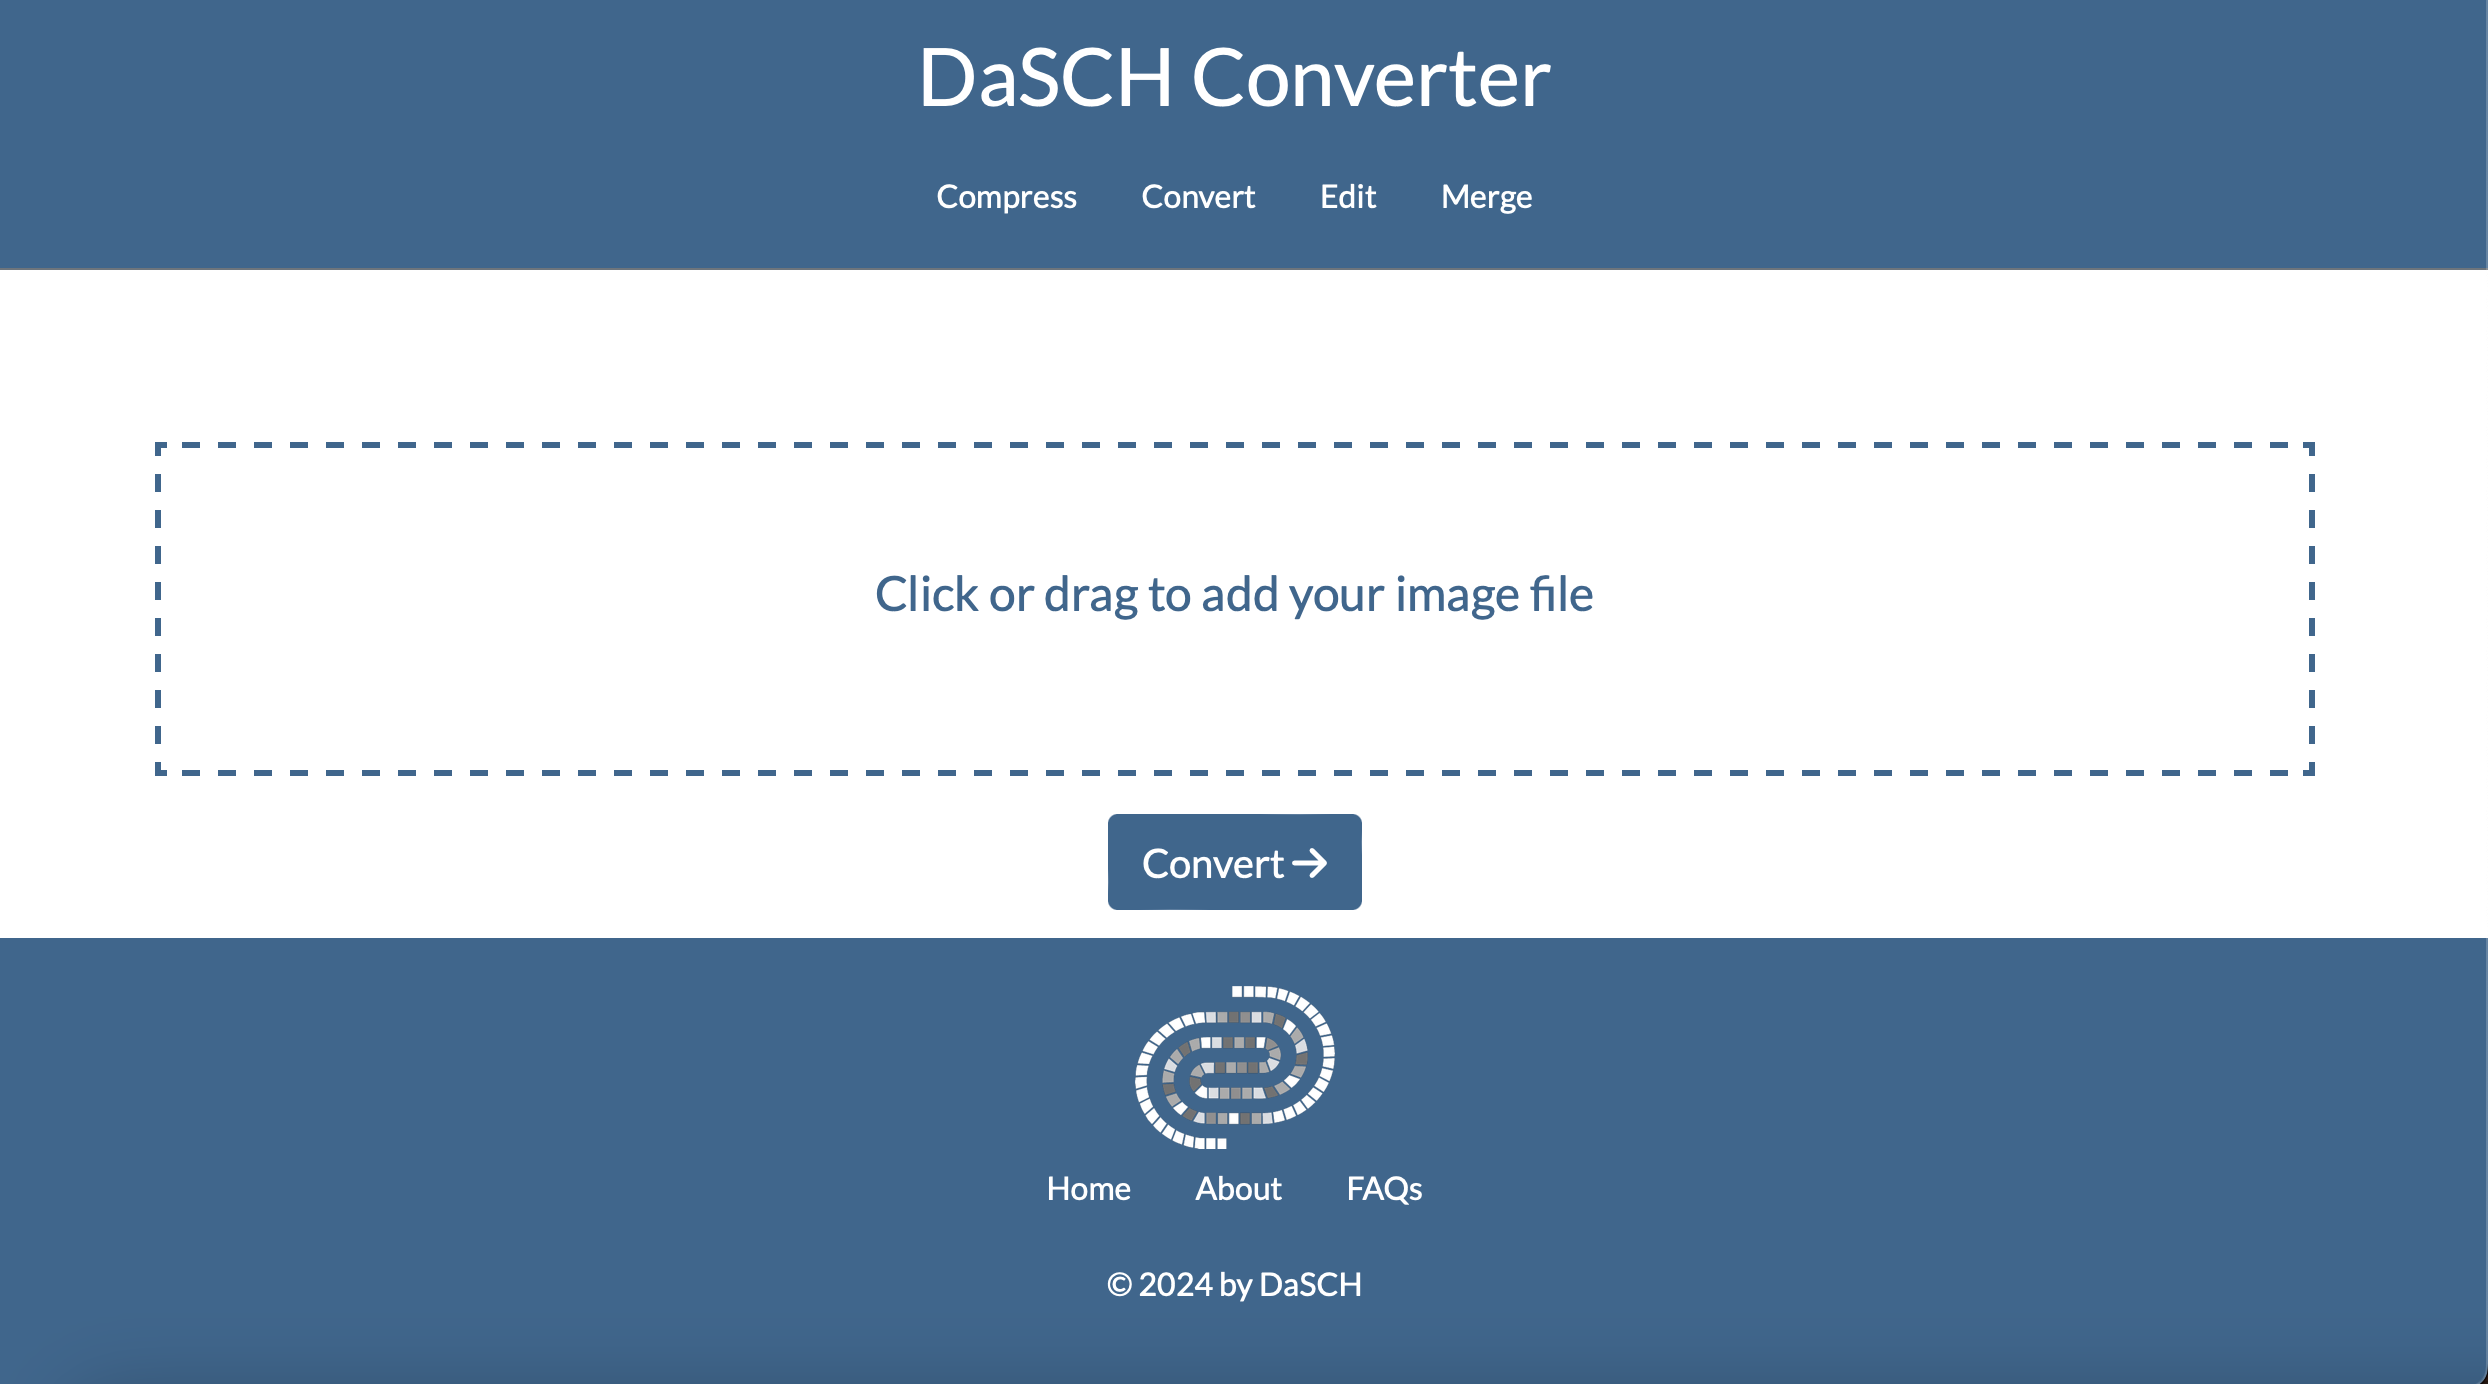
\includegraphics[width=8cm]{02_images/part_02/01_app_dasch_conv.png}
            \caption{Page principale du \cvt}
        \end{figure}

        % home page \msh
        \begin{figure}[h!]
            \centering
            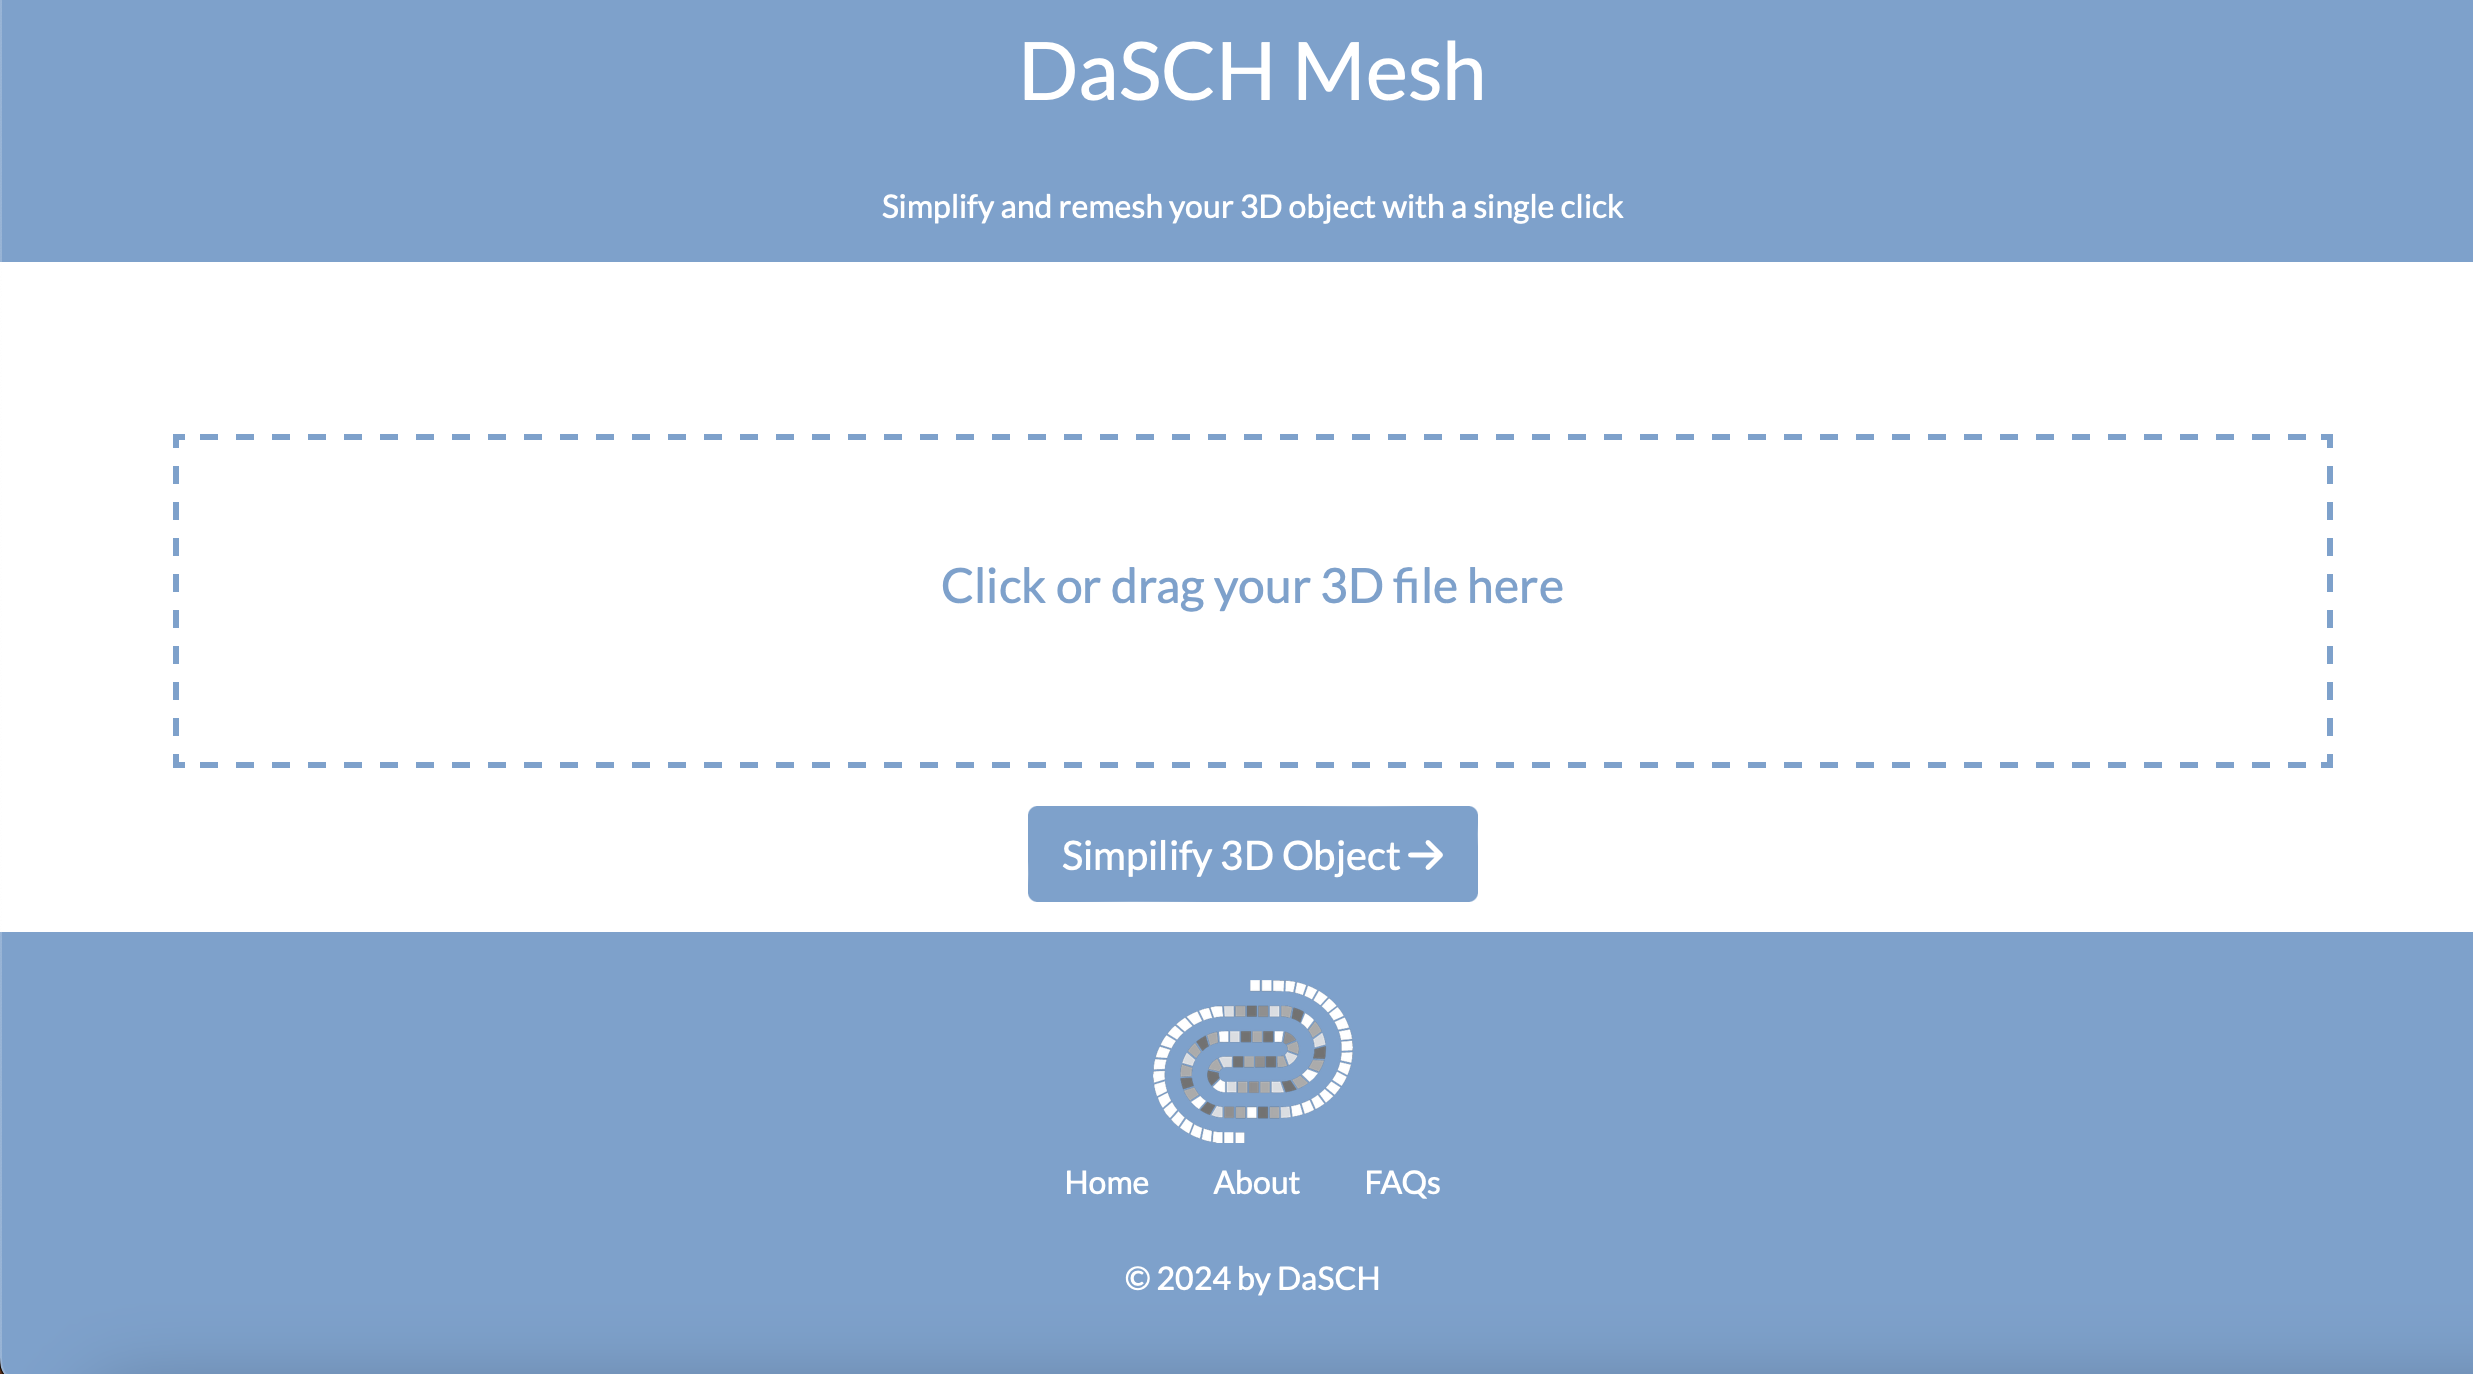
\includegraphics[width=8cm]{02_images/part_02/02_app_dasch_mesh.png}
            \caption{Page principale du \msh}
        \end{figure}
    
        \subsection{Fluidité de l'\ux}
        Enfin, une attention particulière à la fluidité de l'expérience utilisateur a été accordée. Le téléchargement automatique des fichiers une fois la conversion terminée permet de gagner du temps et d'éviter toute manipulation complexe. De plus, l'ensemble des fonctionnalités de l'application a été conçu pour être intuitif et auto-explicatif, ne nécessitant aucune connaissance préalable en informatique de la part de l'utilisateur.

        \subsection{UX et \gco}
        Un UX design minimaliste, caractérisé par une interface épurée et des fonctionnalités essentielles, s'inscrit naturellement dans une démarche éco-responsable. En effet, en réduisant l'encombrement visuel et en simplifiant les interactions, ce type de design contribue à diminuer la charge cognitive des utilisateurs, et aussi pour une prise de décision plus rapide des utilisateurs. Cela se traduit par une consommation moindre de ressources informatiques, telles que la mémoire et la puissance de calcul. De plus, un design minimaliste limite le nombre d'éléments à charger, ce qui optimise la vitesse de chargement des pages et réduit ainsi l'empreinte carbone liée à la consommation énergétique des serveurs.
        
        Enfin, l'intégration de l'\ux dans notre application s'est avérée être un choix stratégique essentiel. En privilégiant la simplicité de fonctionnalités, une courbe d'apprentissage courte et une esthétique soignée, ces applications répondent aux besoins du \dsc. Cet \ux minimaliste en allégeant les applications et en facilitant leur maintenance, permet des codes plus durables, plus accessibles et plus respectueux de l'environnement, tout en offrant une expérience utilisateur optimale. 
        
\chapter{Enrichissement métadonnée : vers les \textit{Scenes} IIIF}
    \section{Conception du \dsc IIIF}
    \diiif est un code \py encore en développement dont le but est enrichir des fichiers 3D avec des métadonnées conformes aux standard IIIF.
        \subsection{Modèles utilisés}
        L'\eng{IIIF Workbench} a été un modèle privilégie afin de regarder la structure base des dossiers contenant des images pour les \eng{Image API} et \eng{Presentation API} d'IIIF, ainsi que pour concevoir un fichier \textsc{json} \footnote{Nous avons utilisé ce site lors du cours \enquote{Anglais langue de l'informatique} dispensé par Edward Gray dans le cadre du master Technologies numériques appliquées à l'histoire à l'\enc. Voir référence \cite{gdmrworkbench}.}.
        
        Ce site nous permet d'envoyer des images qui sont archivées dans nos ordinateurs au site par le biais d'une compte GitHub, auxquels sont associés au \eng{Image API} 2.x ou 3.x. Par la suite, ces images vont avoir un fichier \textsc{json} associé, possédant un \textbf{id} qui permettra, entre autres choses, créer l'\eng{IIIF Manifest}. Dans ce sens, l'\textbf{id} est une information très importante lors de la conceptualisation, et c'est en même temps la caractéristique la plus basique qui autorise à un fichier \textsc{json} devenir un \eng{IIIF Manifest}. Muni de ces deux informations, la modélisation des données est plus profiteuse, une fois que cela montre une application qui enrichie des fichiers avec de métadonnées conformes aux standards d'IIIF.

        \subsection{Prérequis}
        Pour conceptualiser le fichier \textsc{json} avec les paramètres minimaux, le modèle utilisé était extrait de cet exemple d'IIIF \texttt{model\_origin.json} \footnote{Ce modèle minimal pour les modèles 3D, ainsi que d'autres avec plus de paramètres, peuvent être trouvés sur le GitHub d'IIIF. Cf \cite{iiif3dmodelorigin}.}:

        % model_origin.json
        \begin{figure}[h!]
            \centering
            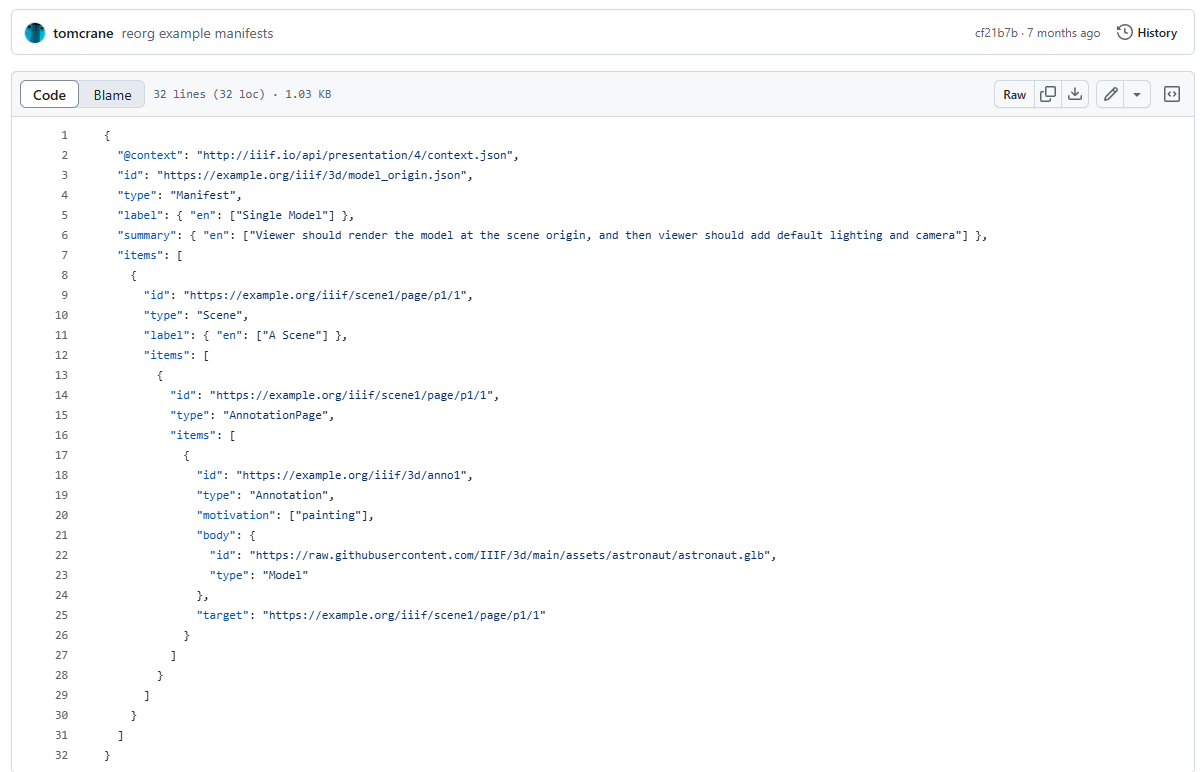
\includegraphics[width=12cm]{02_images/part_02/06_model.png}
            \caption{Code du fichier \texttt{model\_origin.json}}
        \end{figure}

        Il s'agit d'un fichier basique dans lequel force est de constater la présence d'un \texttt{id} qui permet d'utiliser cet objet et le conformer au standard IIIF.
        
        \subsection{Bibliothèques}
        Ce code \py utilise des bibliothèques, tels \textbf{os}, pour concevoir des fichiers \textsc{json}, qui sont les fichiers \eng{Manifest} IIIF, et pour travailler avec les fichiers d'entrée et de sortie.